% questions.tex —— 1977 年·黑龙江卷 · 题目内容片段（无答案）
% 由 tools/generate_projects.py 依来源总账自 1977/1977_数学真题_黑龙江_试题.md 生成，勿手改（改源 MD 后重跑）


\gkpart{数学试卷（黑龙江卷）}

\begin{gktip}
\textbf{来源说明}：本题面依据固定源 PDF《1977 黑龙江卷数学试卷》第 1 页逐题转录。源文件为上游重新排版的 TeX 版 A3 单页（非原始扫描卷），原卷未附答案页；配套答案与解析为本库编者独立推导，\textbf{非官方标准答案}。原卷卷首印有编注：「文科做 1-7，理科做 2-8，9 附加题 20 分，10 参考题不计入总分」，正式题按编注取第 1—8 题，附加题 9 与参考题 10 不计入正式题量。第 5、9 题的几何图按源卷原图重绘。
\end{gktip}

\par\medskip

\begin{question}
\gkti{1}解答下列各题：

（1） 解方程：$\sqrt{3x+4}=4$。

（2） 解不等式：$|x|<5$。

（3） 已知正三角形的外接圆半径为 $6\sqrt3\ \mathrm{cm}$，求它的边长。

\end{question}
\begin{question}
\gkti{2}计算下列各题：

（1） $\sqrt{m^2-2ma+a^2}$。

（2） $\cos78^\circ\cdot\cos3^\circ+\cos12^\circ\cdot\sin3^\circ$。

（3） $\arcsin\left(\cos\dfrac{\pi}{6}\right)$。

\end{question}
\begin{question}
\gkti{3}解下列各题：

（1） 解方程：$3^{x+1}-9^{\frac{x}{2}}=18$。

（2） 求数列 $2,4,8,16,\cdots$ 前十项的和。

\end{question}
\begin{question}
\gkti{4}解下列各题：

（1） 圆锥的高为 $6\ \mathrm{cm}$，母线和底面半径成 $30^\circ$ 角，求它的侧面积。

（2） 求过点 $(1,4)$ 且与直线 $2x-5y+3=0$ 垂直的直线方程。

\Needspace{0.4\textheight}
\end{question}
\begin{question}
\gkti{5}如果 $\triangle ABC$ 的 $\angle A$ 的平分线交 $BC$ 于 $D$，交它的外接圆于 $E$，那么 $AB\cdot AC=AD\cdot AE$。
\nopagebreak[4]
\begin{center}% 1977 年黑龙江卷第 5 题：△ABC 内接于圆，∠A 的平分线 AE 交 BC 于 D、交外接圆于 E（按源卷布局）
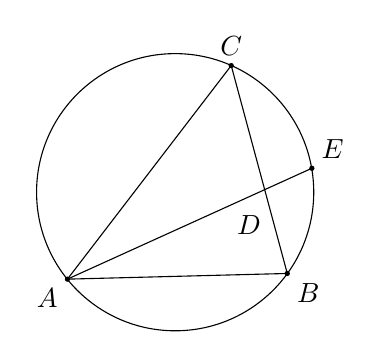
\begin{tikzpicture}[scale=0.8]
  \draw (0,0) circle (2.2);
  \coordinate (A) at (-1.71,-1.38);
  \coordinate (B) at (1.78,-1.29);
  \coordinate (C) at (0.89,2.01);
  \coordinate (E) at (2.17,0.38);
  \coordinate (D) at (1.42,0.04);
  \draw (A) -- (B) -- (C) -- cycle;
  \draw (A) -- (E);
  \fill (A) circle (1.2pt) node[below left] {$A$};
  \fill (B) circle (1.2pt) node[below right] {$B$};
  \fill (C) circle (1.2pt) node[above] {$C$};
  \fill (E) circle (1.2pt) node[above right] {$E$};
  \node at (1.17,-0.52) {$D$};
\end{tikzpicture}
\end{center}
\nopagebreak[4]
\end{question}
\begin{question}
\gkti{6}前进大队响应毛主席关于“绿化祖国”的伟大号召，1975 年造林 200 亩，又知 1975 年至 1977 年这三年内共造林 728 亩，求后两年造林面积的年平均增长率是多少？

\end{question}
\begin{question}
\gkti{7}解方程：$\lg(2^x+2x-16)=x(1-\lg5)$。

\Needspace{0.4\textheight}
\end{question}
\begin{question}
\gkti{8}已知三角形的三边成等差数列，周长为 $36\ \mathrm{cm}$，面积为 $54\ \mathrm{cm^2}$，求三边的长。

\begin{gktip}
\Needspace{0.25\textheight}
\textbf{附加题}
\end{gktip}

\textbf{附加题 9．（20 分）} 如图，$AP$ 表示发动机的连杆，$OA$ 表示它的曲柄。当 $A$ 在圆上作圆周运动时，$P$ 在 $x$ 轴上作直线运动，求 $P$ 点的横坐标。为什么当 $\alpha$ 是直角时，$\angle P$ 是最大？
\nopagebreak[4]
\begin{center}% 1977 年黑龙江卷附加题第 9 题：曲柄连杆机构，圆心 O、曲柄 OA（半径 R）、
% 连杆 AP（l）、曲柄转角 α 标在 O 处，P 在 x 轴上（按源卷布局）
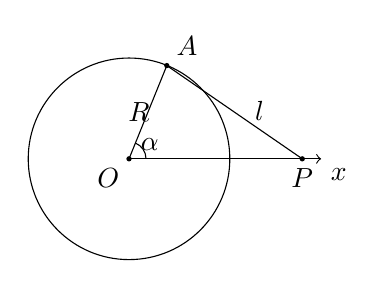
\begin{tikzpicture}[scale=0.8]
  \draw (0,0) circle (1.6);
  \coordinate (O) at (0,0);
  \coordinate (A) at (0.60,1.48);
  \coordinate (P) at (2.75,0);
  \draw[->] (0,0) -- (3.05,0) node[below right] {$x$};
  \draw (O) -- (A);
  \draw (A) -- (P);
  \draw (0.27,0) arc (0:68:0.27);
  \fill (O) circle (1.2pt) node[below left] {$O$};
  \fill (A) circle (1.2pt) node[above right] {$A$};
  \fill (P) circle (1.2pt) node[below] {$P$};
  \node at (0.16,0.75) {$R$};
  \node at (2.07,0.76) {$l$};
  \node at (0.33,0.22) {$\alpha$};
\end{tikzpicture}
\end{center}
\nopagebreak[4]
\textbf{参考题 10．} 求曲线 $y=\sin x$ 在 $[0,\pi]$ 上的曲边梯形绕 $x$ 轴旋转一周所形成的旋转体的体积。

\end{question}